\begin{figure}[H]
\centering
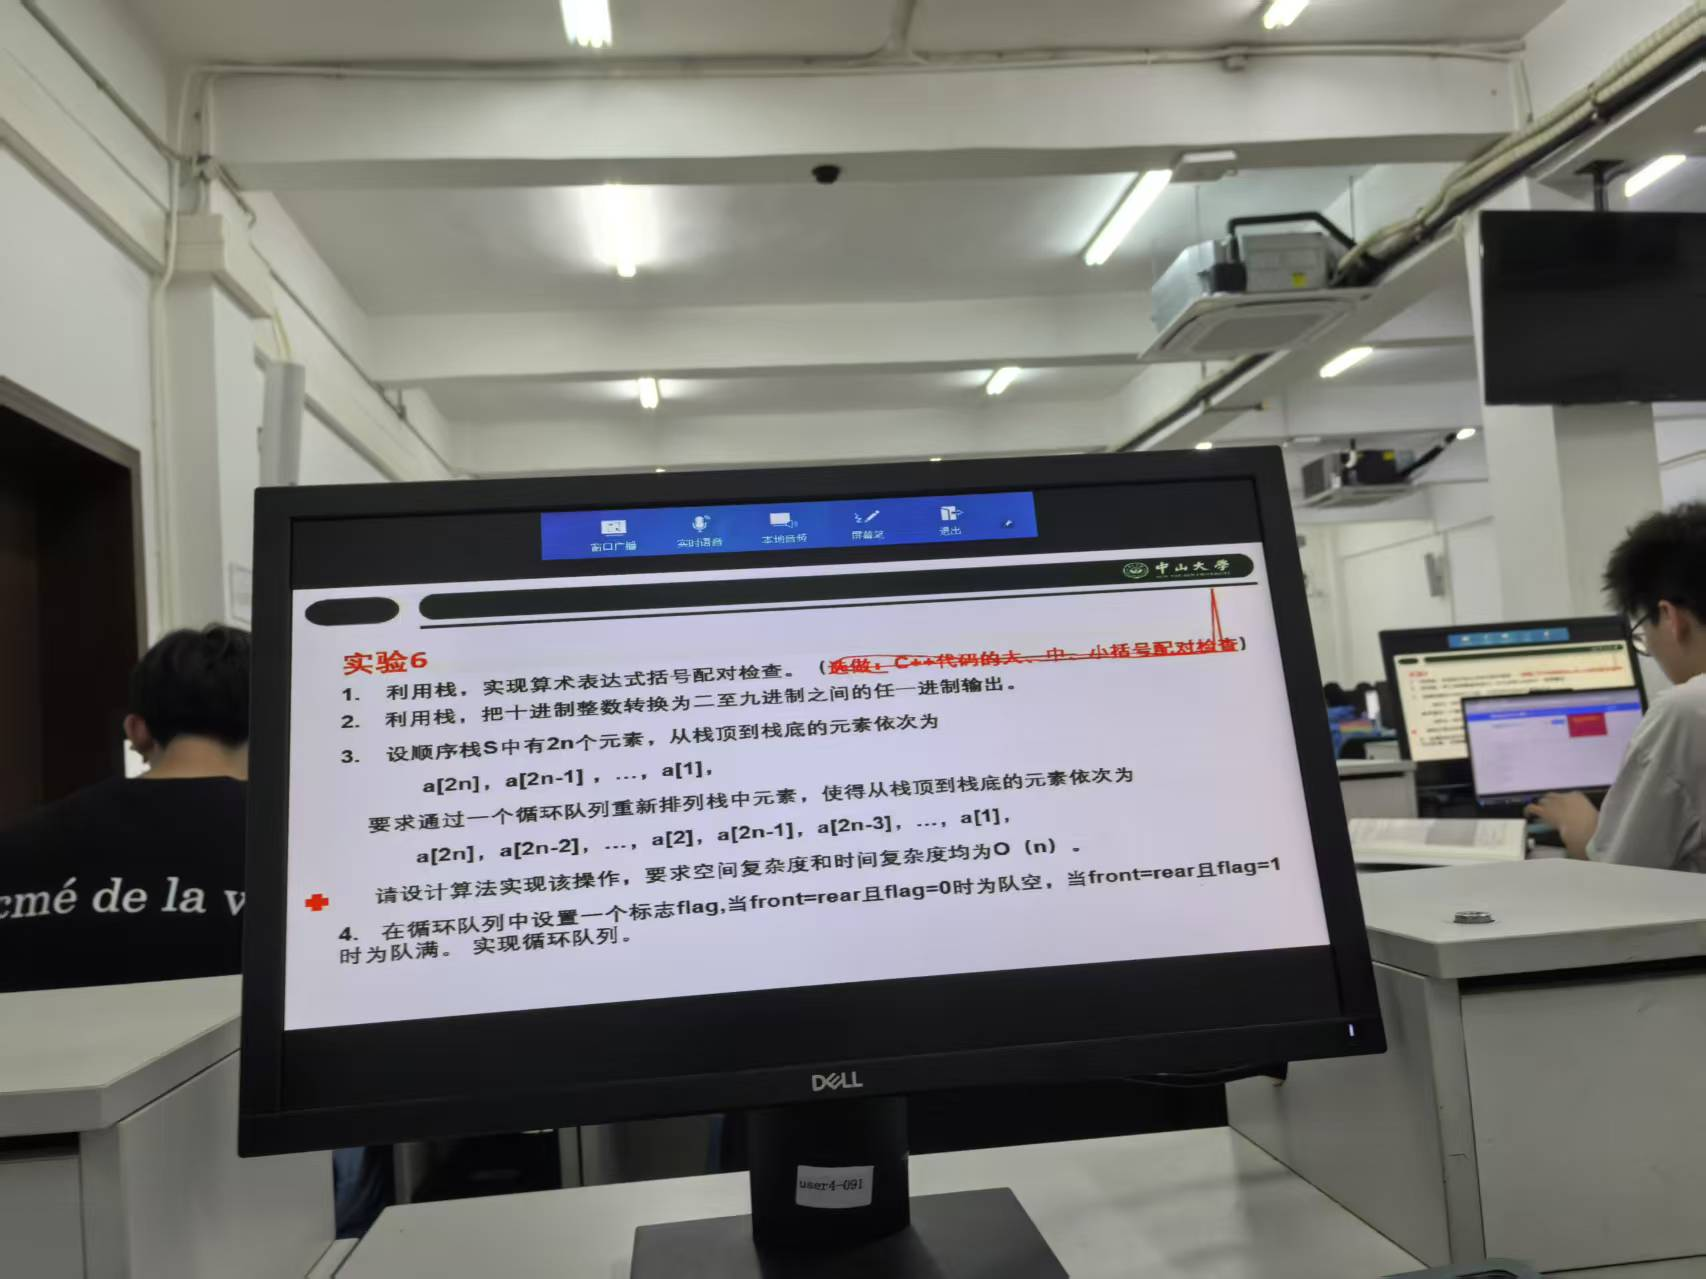
\includegraphics[width=\textwidth]{0.jpg}
% \caption{}
\label{}
\end{figure}

\section{利用栈,实现算数表达式符号配对检查}

\begin{figure}[H]
\centering
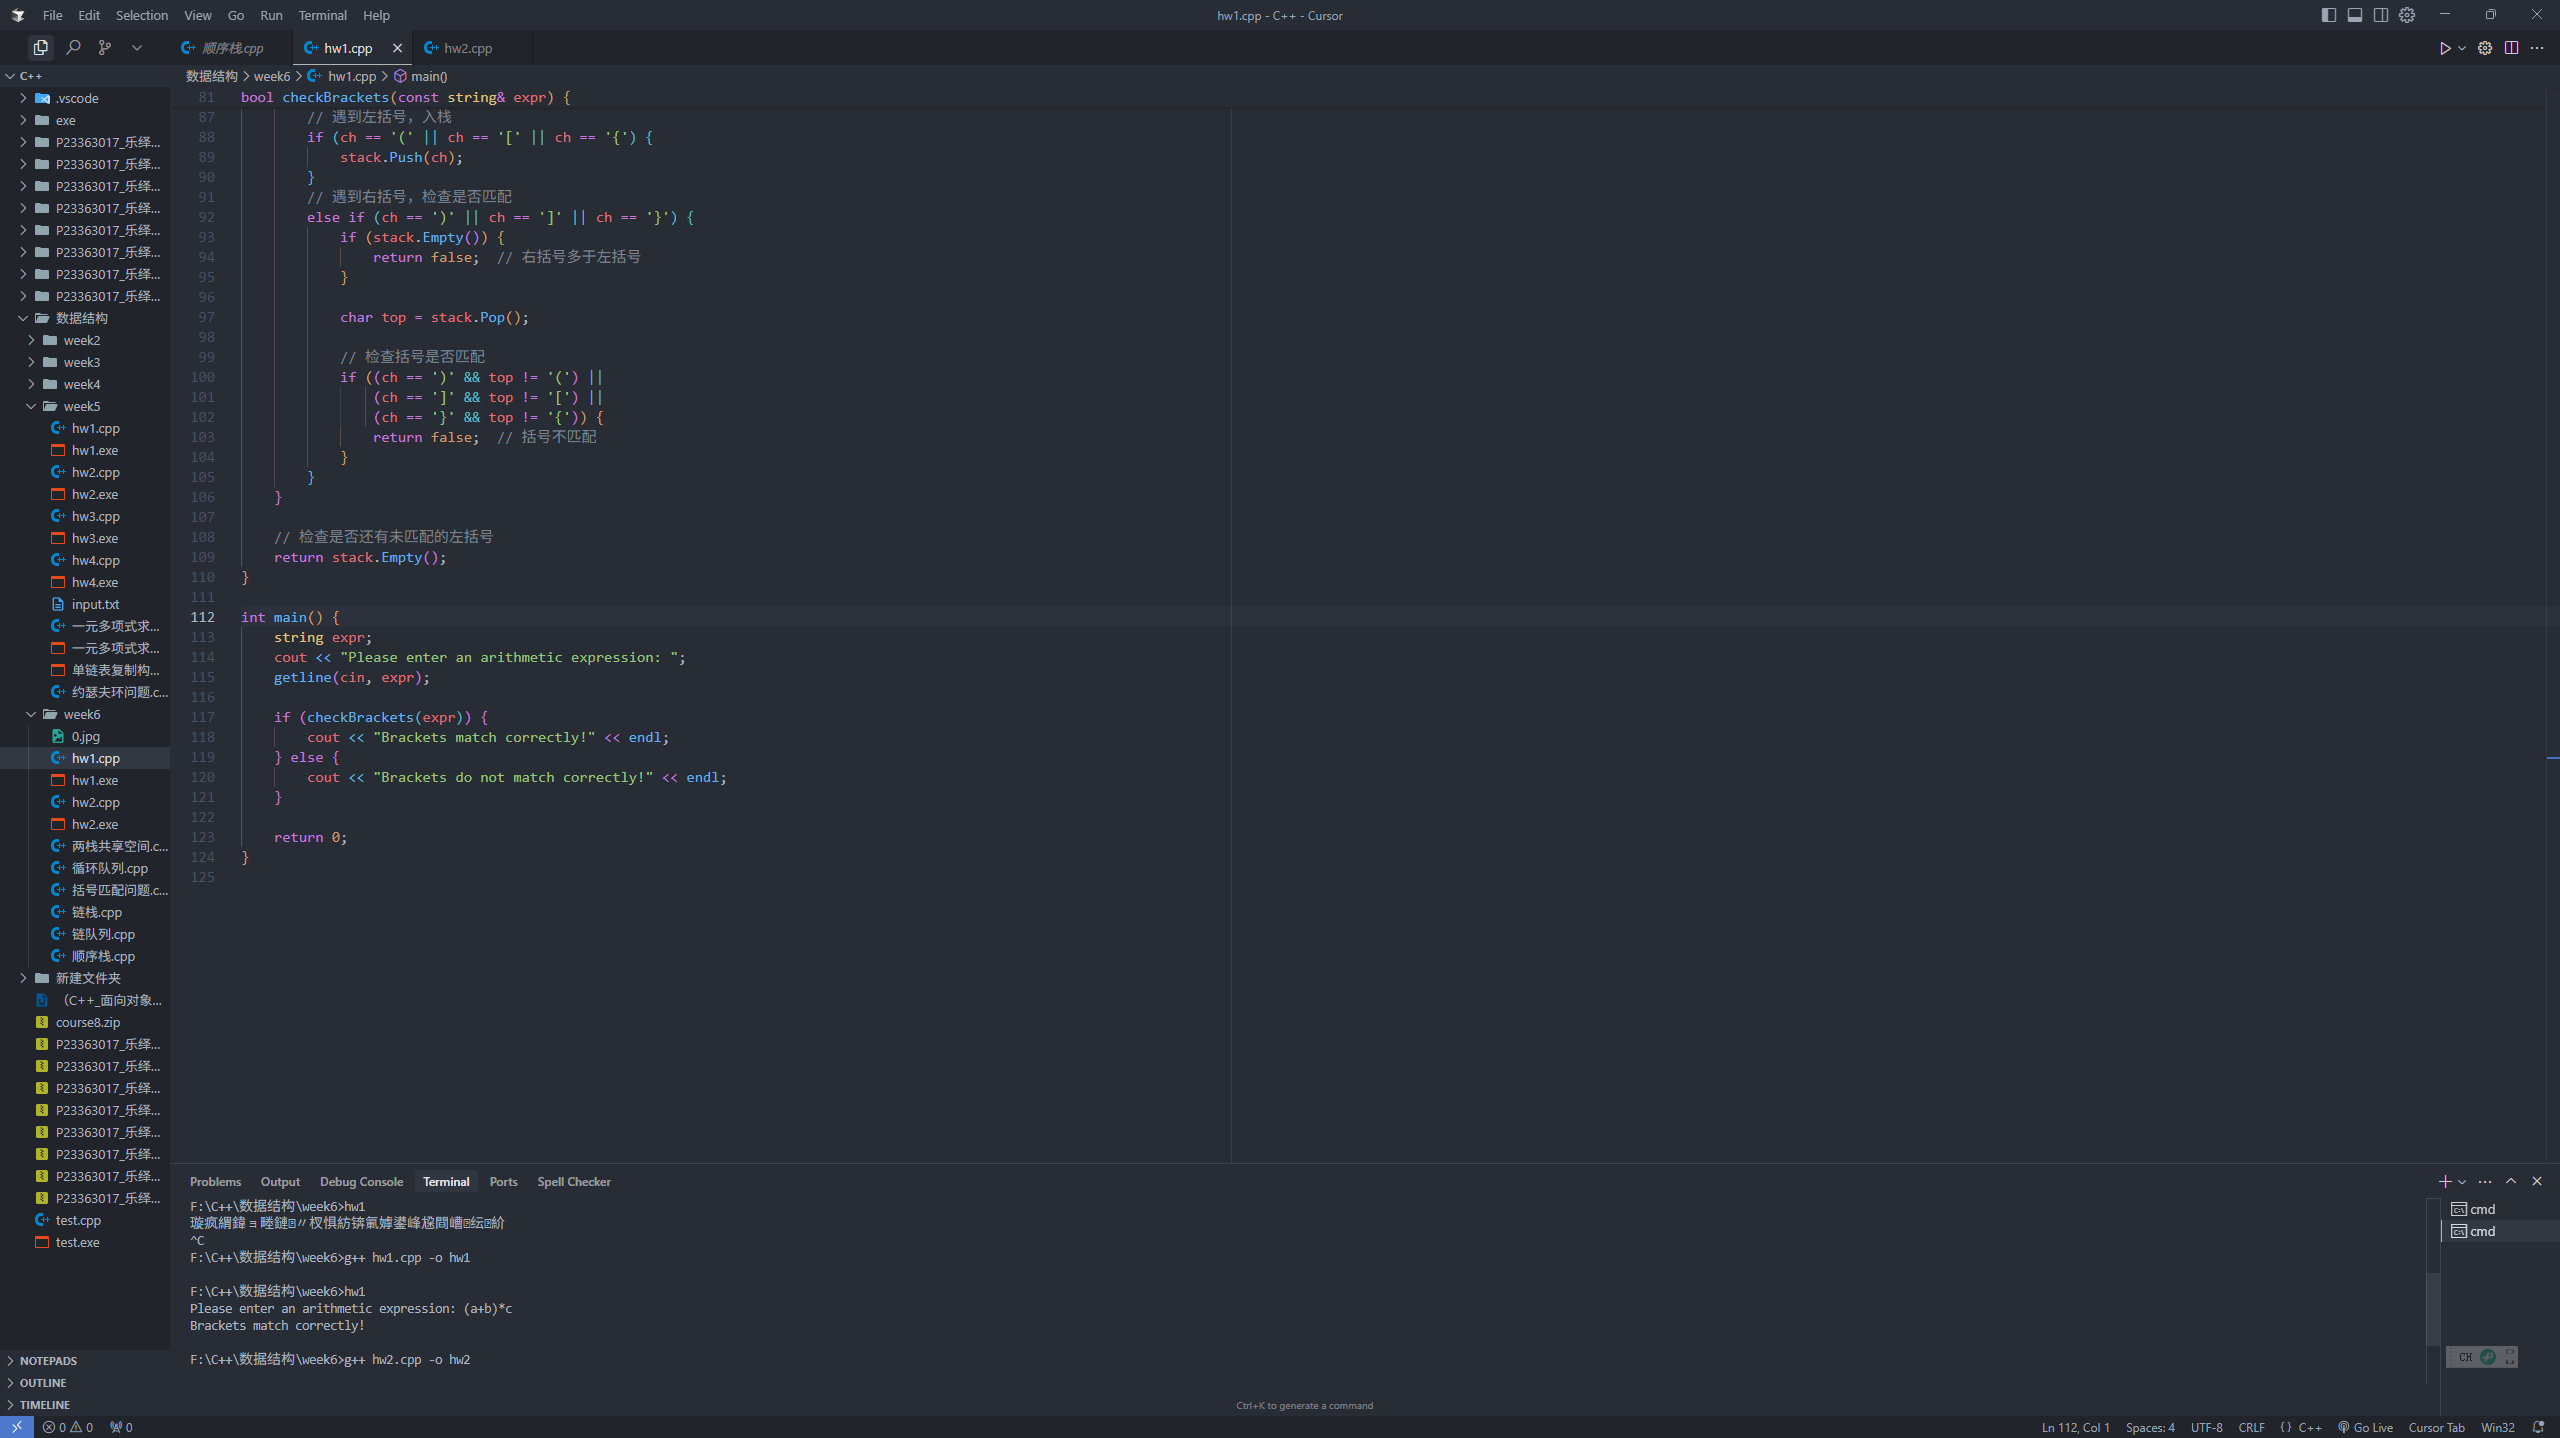
\includegraphics[width=\textwidth]{1-实验报告6-2025041423.png}
% \caption{}
\label{}
\end{figure}

\begin{lstlisting}[language=C++]
#include <iostream>

#include <string>

using namespace std;

  

// 定义链栈节点结构

template <typename DataType>

struct Node {

    DataType data;

    Node<DataType> *next;

};

  

// 定义链栈类

template <typename DataType>

class LinkStack {

public:

    LinkStack();                     // 构造函数

    ~LinkStack();                    // 析构函数

    void Push(DataType x);           // 入栈操作

    DataType Pop();                  // 出栈操作

    DataType GetTop();               // 获取栈顶元素

    int Empty();                     // 判断栈是否为空

private:

    Node<DataType> *top;             // 栈顶指针

};

  

// 构造函数

template <typename DataType>

LinkStack<DataType>::LinkStack() {

    top = NULL;

}

  

// 析构函数

template <typename DataType>

LinkStack<DataType>::~LinkStack() {

    Node<DataType> *q = NULL;

    while (top != NULL) {

        q = top;

        top = top->next;

        delete q;

    }

}

  

// 入栈操作

template <typename DataType>

void LinkStack<DataType>::Push(DataType x) {

    Node<DataType> *s = new Node<DataType>;

    s->data = x;

    s->next = top;

    top = s;

}

  

// 出栈操作

template <typename DataType>

DataType LinkStack<DataType>::Pop() {

    if (Empty())

        throw "栈为空,无法出栈";

    DataType x = top->data;

    Node<DataType> *p = top;

    top = top->next;

    delete p;

    return x;

}

  

// 获取栈顶元素

template <typename DataType>

DataType LinkStack<DataType>::GetTop() {

    if (Empty())

        throw "栈为空,无法获取栈顶元素";

    return top->data;

}

  

// 判断栈是否为空

template <typename DataType>

int LinkStack<DataType>::Empty() {

    return top == NULL;

}

  

// 检查表达式中的括号是否匹配

bool checkBrackets(const string& expr) {

    LinkStack<char> stack;

    for (size_t i = 0; i < expr.length(); i++) {

        char ch = expr[i];

        // 遇到左括号,入栈

        if (ch == '(' || ch == '[' || ch == '{') {

            stack.Push(ch);

        }

        // 遇到右括号,检查是否匹配

        else if (ch == ')' || ch == ']' || ch == '}') {

            if (stack.Empty()) {

                return false;  // 右括号多于左括号

            }

            char top = stack.Pop();

            // 检查括号是否匹配

            if ((ch == ')' && top != '(') ||

                (ch == ']' && top != '[') ||

                (ch == '}' && top != '{')) {

                return false;  // 括号不匹配

            }

        }

    }

    // 检查是否还有未匹配的左括号

    return stack.Empty();

}

  

int main() {

    string expr;

    cout << "Please enter an arithmetic expression: ";

    getline(cin, expr);

    if (checkBrackets(expr)) {

        cout << "Brackets match correctly!" << endl;

    } else {

        cout << "Brackets do not match correctly!" << endl;

    }

    return 0;

}
\end{lstlisting}
\section{利用栈,把十进制整数转换为二至九进制之间的任一进制输出}

\begin{figure}[H]
\centering
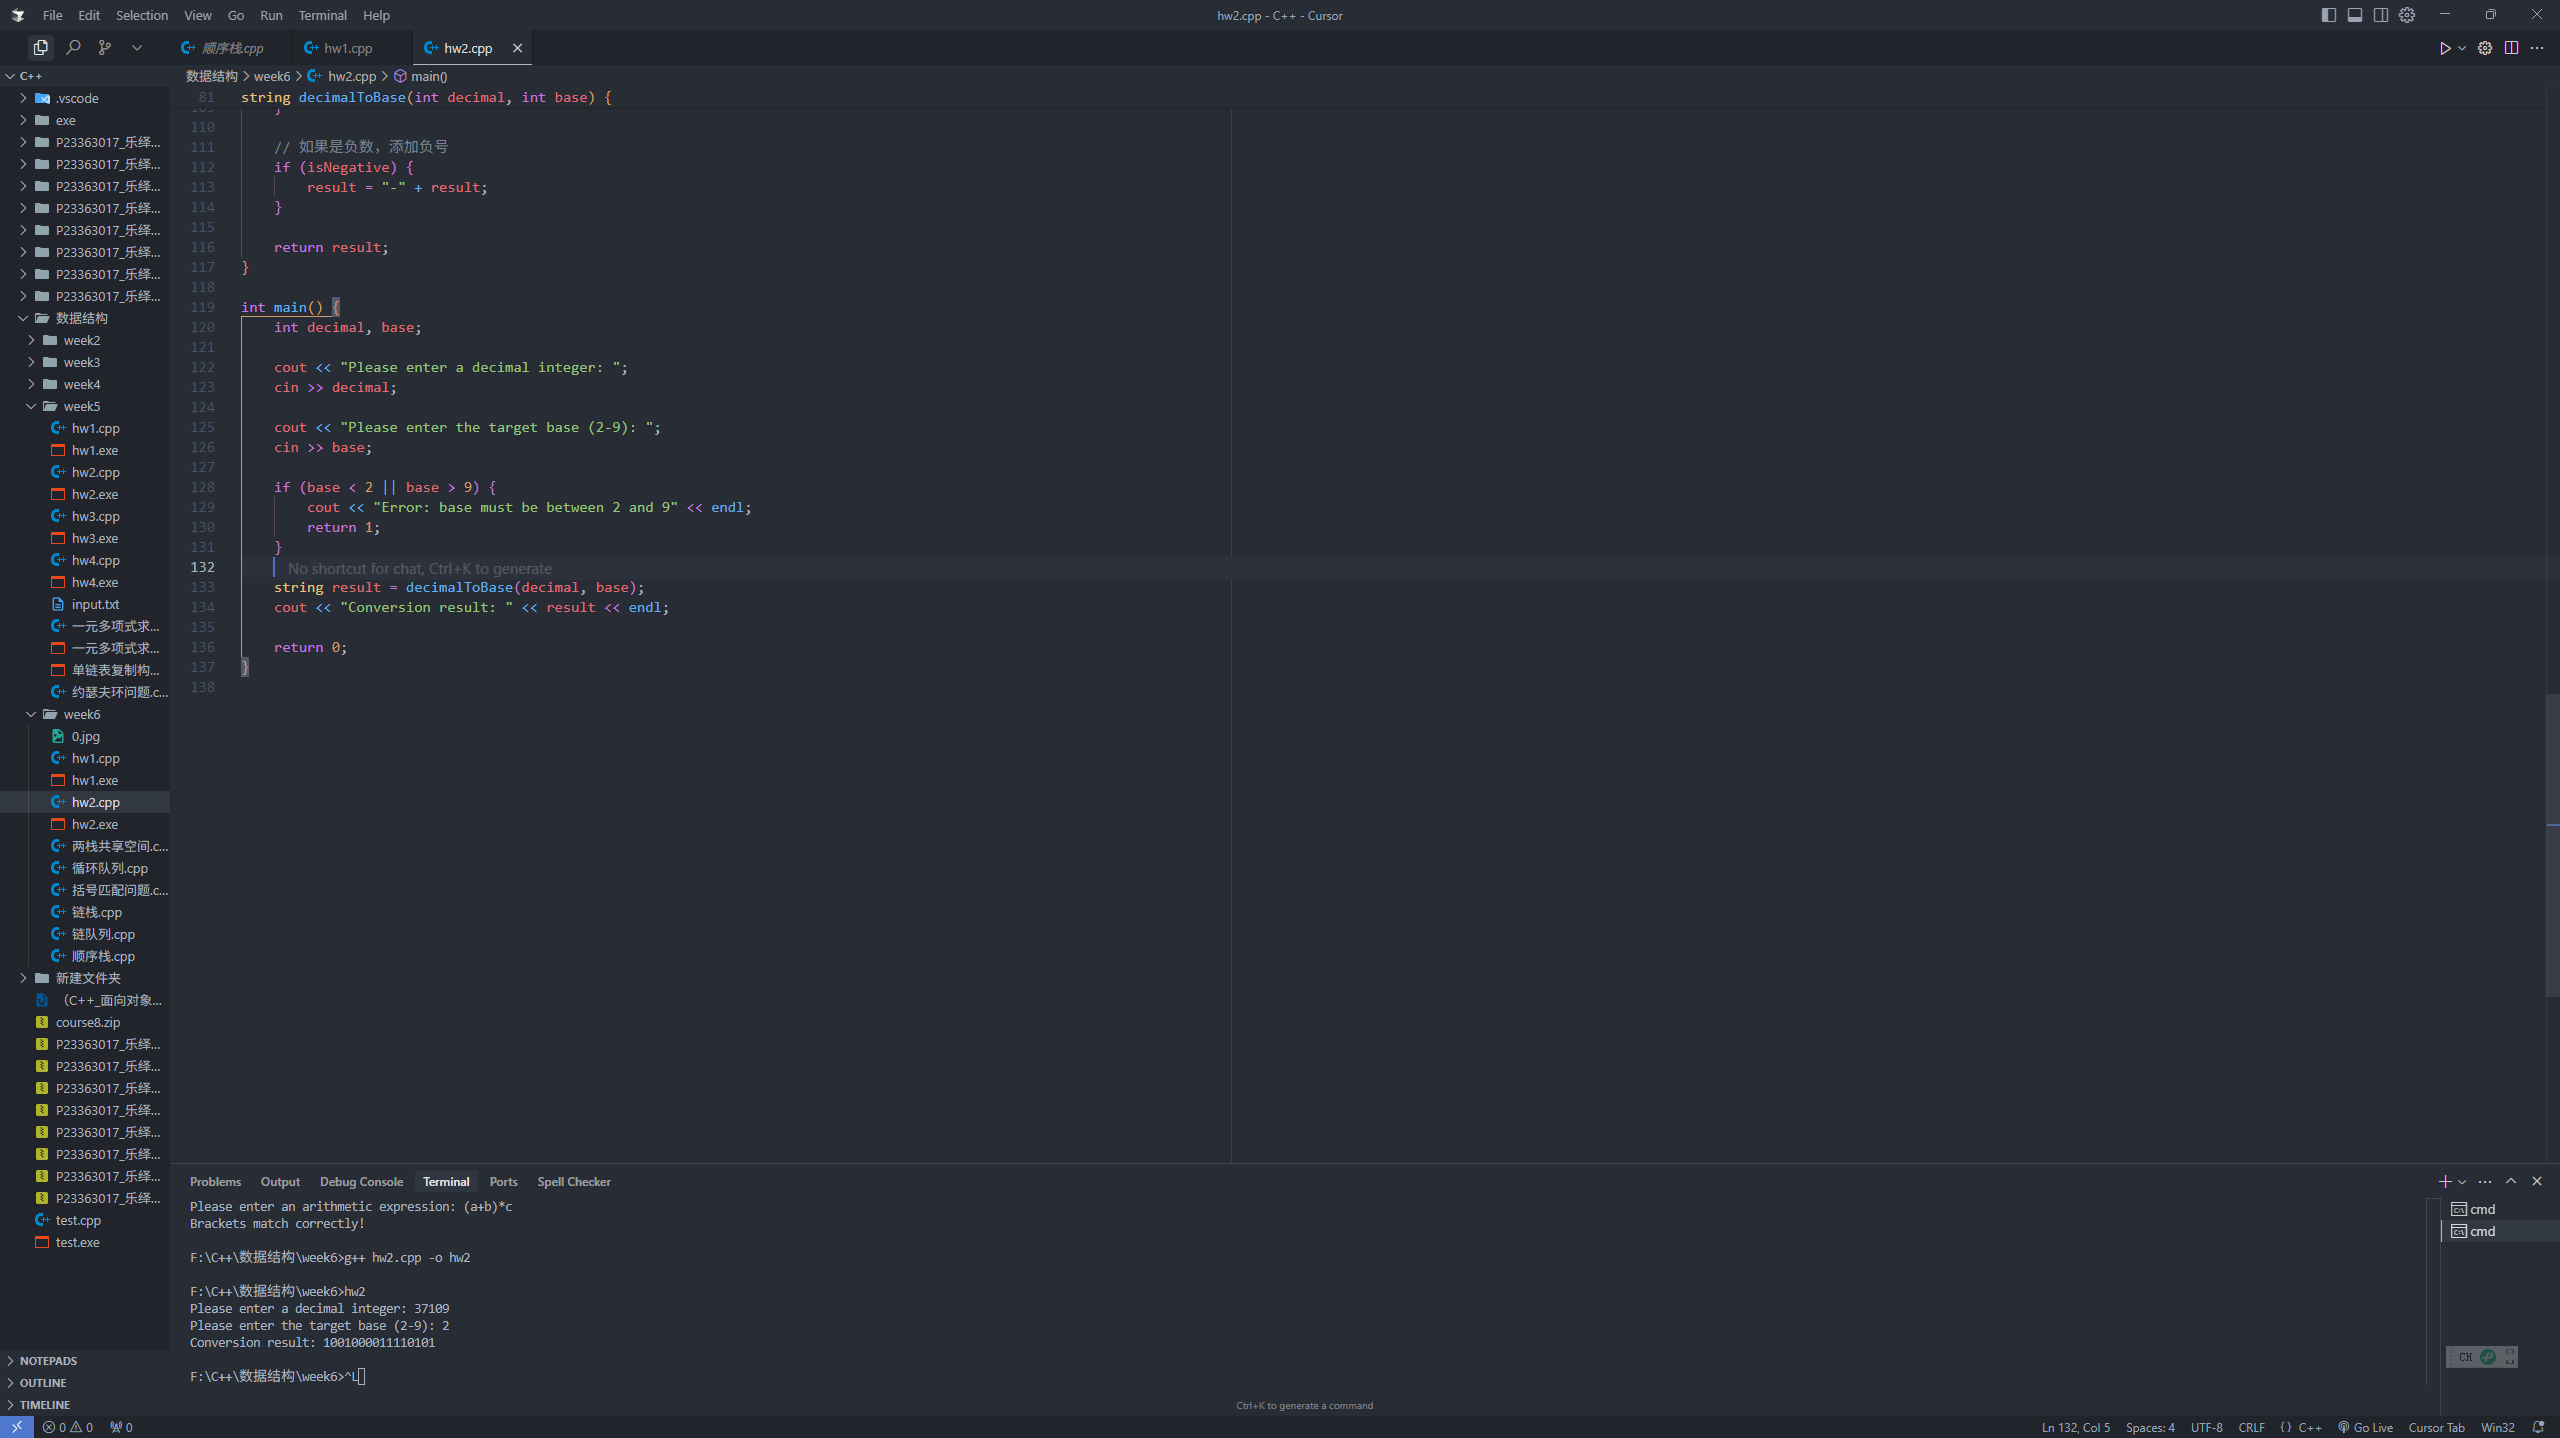
\includegraphics[width=\textwidth]{实验报告6-2025041423.png}
% \caption{}
\label{}
\end{figure}

\begin{lstlisting}[language=C++]
#include <iostream>

#include <string>

using namespace std;

  

// 定义链栈节点结构

template <typename DataType>

struct Node {

    DataType data;

    Node<DataType> *next;

};

  

// 定义链栈类

template <typename DataType>

class LinkStack {

public:

    LinkStack();                     // 构造函数

    ~LinkStack();                    // 析构函数

    void Push(DataType x);           // 入栈操作

    DataType Pop();                  // 出栈操作

    DataType GetTop();               // 获取栈顶元素

    int Empty();                     // 判断栈是否为空

private:

    Node<DataType> *top;             // 栈顶指针

};

  

// 构造函数

template <typename DataType>

LinkStack<DataType>::LinkStack() {

    top = NULL;

}

  

// 析构函数

template <typename DataType>

LinkStack<DataType>::~LinkStack() {

    Node<DataType> *q = NULL;

    while (top != NULL) {

        q = top;

        top = top->next;

        delete q;

    }

}

  

// 入栈操作

template <typename DataType>

void LinkStack<DataType>::Push(DataType x) {

    Node<DataType> *s = new Node<DataType>;

    s->data = x;

    s->next = top;

    top = s;

}

  

// 出栈操作

template <typename DataType>

DataType LinkStack<DataType>::Pop() {

    if (Empty())

        throw "栈为空,无法出栈";

    DataType x = top->data;

    Node<DataType> *p = top;

    top = top->next;

    delete p;

    return x;

}

  

// 获取栈顶元素

template <typename DataType>

DataType LinkStack<DataType>::GetTop() {

    if (Empty())

        throw "栈为空,无法获取栈顶元素";

    return top->data;

}

  

// 判断栈是否为空

template <typename DataType>

int LinkStack<DataType>::Empty() {

    return top == NULL;

}

  

// 十进制转换为指定进制

string decimalToBase(int decimal, int base) {

    if (base < 2 || base > 9) {

        return "进制范围应为2-9";

    }

    if (decimal == 0) {

        return "0";

    }

    LinkStack<int> stack;

    string result = "";

    // 处理负数

    bool isNegative = false;

    if (decimal < 0) {

        isNegative = true;

        decimal = -decimal;

    }

    // 进行进制转换

    while (decimal > 0) {

        stack.Push(decimal % base);

        decimal /= base;

    }

    // 从栈中弹出结果

    while (!stack.Empty()) {

        result += to_string(stack.Pop());

    }

    // 如果是负数,添加负号

    if (isNegative) {

        result = "-" + result;

    }

    return result;

}

  

int main() {

    int decimal, base;

    cout << "Please enter a decimal integer: ";

    cin >> decimal;

    cout << "Please enter the target base (2-9): ";

    cin >> base;

    if (base < 2 || base > 9) {

        cout << "Error: base must be between 2 and 9" << endl;

        return 1;

    }

    string result = decimalToBase(decimal, base);

    cout << "Conversion result: " << result << endl;

    return 0;

}
\end{lstlisting}
\section{通过循环队列重新排列战中元素}

\begin{figure}[H]
\centering
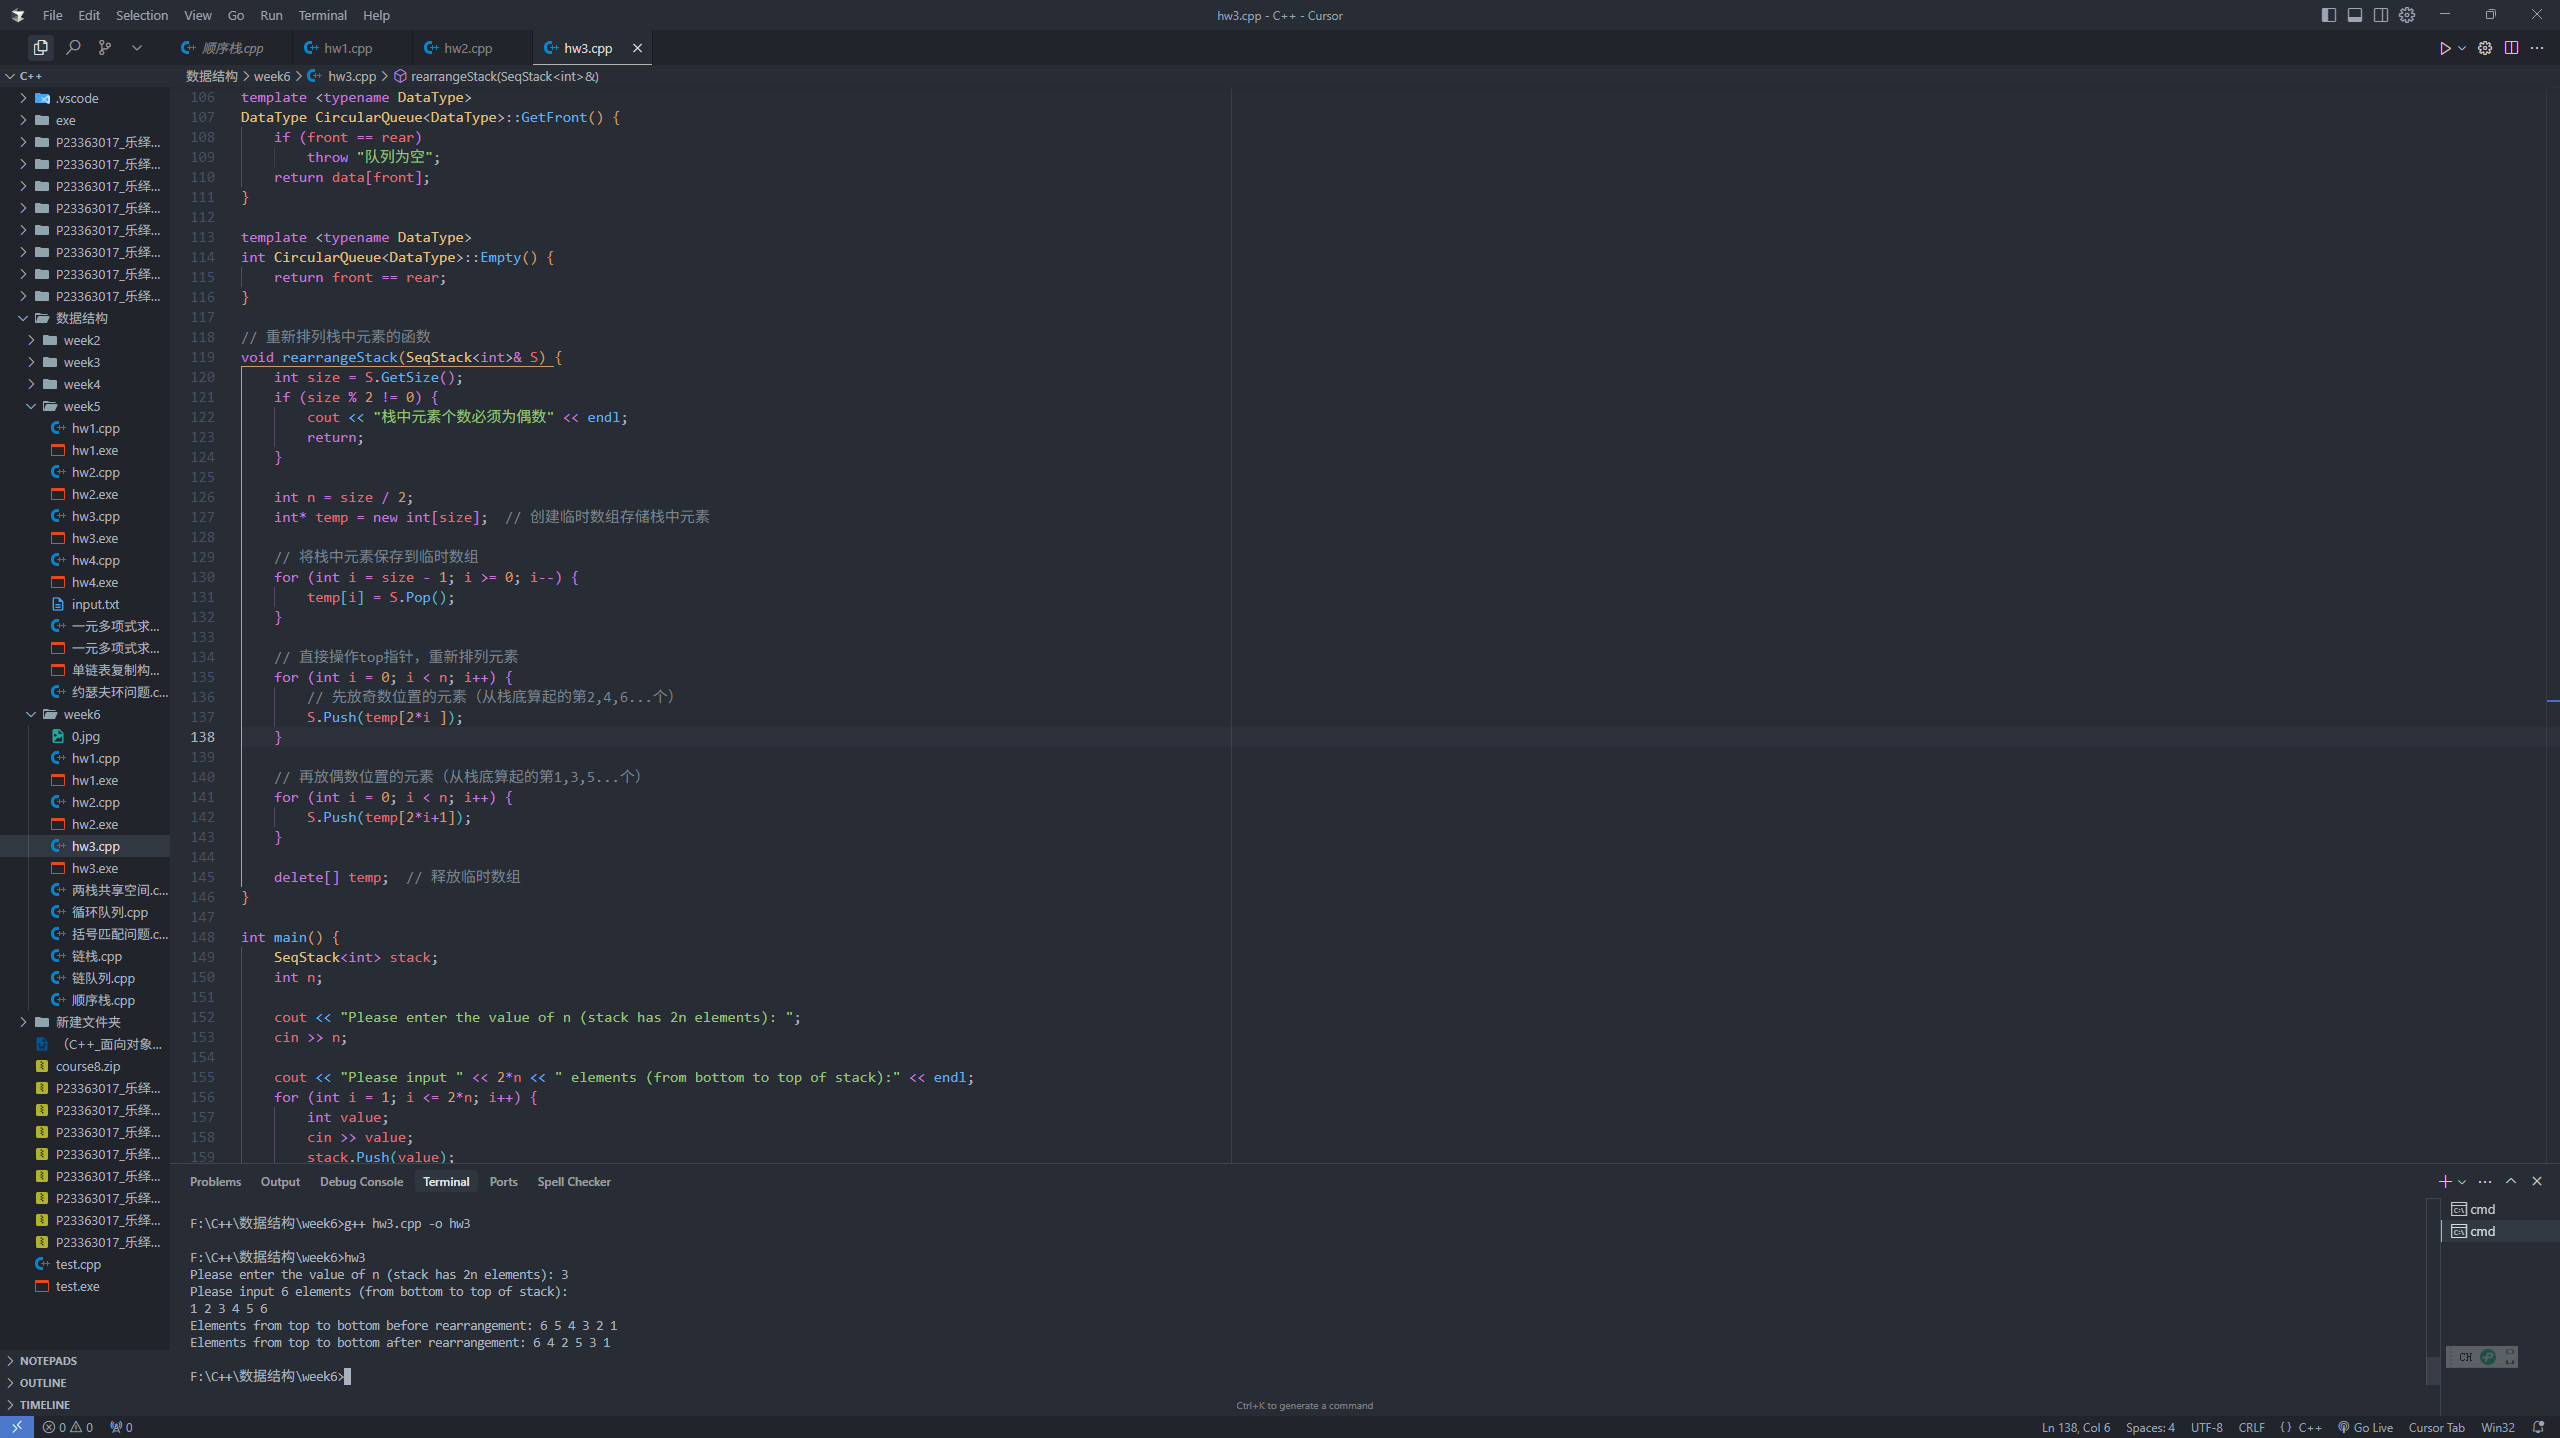
\includegraphics[width=\textwidth]{2-实验报告6-2025041423.png}
% \caption{}
\label{}
\end{figure}

\begin{lstlisting}[language=C++]
#include <iostream>

using namespace std;

  

const int StackSize = 100;  // 栈的最大容量

const int QueueSize = 100;  // 队列的最大容量

  

// 顺序栈类定义

template <typename DataType>

class SeqStack {

public:

    SeqStack();                  // 构造函数

    ~SeqStack();                 // 析构函数

    void Push(DataType x);       // 入栈操作

    DataType Pop();              // 出栈操作

    DataType GetTop();           // 获取栈顶元素

    int Empty();                 // 判断栈是否为空

    int GetSize();               // 获取栈中元素个数

private:

    DataType data[StackSize];    // 存放栈元素的数组

    int top;                     // 栈顶指针

};

  

// 循环队列类定义

template <typename DataType>

class CircularQueue {

public:

    CircularQueue();             // 构造函数

    ~CircularQueue();            // 析构函数

    void EnQueue(DataType x);    // 入队操作

    DataType DeQueue();          // 出队操作

    DataType GetFront();         // 获取队头元素

    int Empty();                 // 判断队列是否为空

private:

    DataType data[QueueSize];    // 存放队列元素的数组

    int front, rear;             // 队头和队尾指针

};

  

// 顺序栈的实现

template <typename DataType>

SeqStack<DataType>::SeqStack() {

    top = -1;

}

  

template <typename DataType>

SeqStack<DataType>::~SeqStack() {

}

  

template <typename DataType>

void SeqStack<DataType>::Push(DataType x) {

    if (top == StackSize - 1)

        throw "栈上溢";

    data[++top] = x;

}

  

template <typename DataType>

DataType SeqStack<DataType>::Pop() {

    if (top == -1)

        throw "栈下溢";

    return data[top--];

}

  

template <typename DataType>

DataType SeqStack<DataType>::GetTop() {

    if (top == -1)

        throw "栈为空";

    return data[top];

}

  

template <typename DataType>

int SeqStack<DataType>::Empty() {

    return top == -1;

}

  

template <typename DataType>

int SeqStack<DataType>::GetSize() {

    return top + 1;

}

  

// 循环队列的实现

template <typename DataType>

CircularQueue<DataType>::CircularQueue() {

    front = rear = 0;

}

  

template <typename DataType>

CircularQueue<DataType>::~CircularQueue() {

}

  

template <typename DataType>

void CircularQueue<DataType>::EnQueue(DataType x) {

    if ((rear + 1) % QueueSize == front)

        throw "队列上溢";

    data[rear] = x;

    rear = (rear + 1) % QueueSize;

}

  

template <typename DataType>

DataType CircularQueue<DataType>::DeQueue() {

    if (front == rear)

        throw "队列下溢";

    DataType x = data[front];

    front = (front + 1) % QueueSize;

    return x;

}

  

template <typename DataType>

DataType CircularQueue<DataType>::GetFront() {

    if (front == rear)

        throw "队列为空";

    return data[front];

}

  

template <typename DataType>

int CircularQueue<DataType>::Empty() {

    return front == rear;

}

  

// 重新排列栈中元素的函数

void rearrangeStack(SeqStack<int>& S) {

    int size = S.GetSize();

    if (size % 2 != 0) {

        cout << "栈中元素个数必须为偶数" << endl;

        return;

    }

    int n = size / 2;

    int* temp = new int[size];  // 创建临时数组存储栈中元素

    // 将栈中元素保存到临时数组

    for (int i = size - 1; i >= 0; i--) {

        temp[i] = S.Pop();

    }

    // 直接操作top指针,重新排列元素

    for (int i = 0; i < n; i++) {

        // 先放奇数位置的元素(从栈底算起的第1,3,5...个)

        S.Push(temp[2*i ]);

    }

    // 再放偶数位置的元素(从栈底算起的第2,4,6...个)

    for (int i = 0; i < n; i++) {

        S.Push(temp[2*i+1]);

    }

    delete[] temp;  // 释放临时数组

}

  

int main() {

    SeqStack<int> stack;

    int n;

    cout << "Please enter the value of n (stack has 2n elements): ";

    cin >> n;

    cout << "Please input " << 2*n << " elements (from bottom to top of stack):" << endl;

    for (int i = 1; i <= 2*n; i++) {

        int value;

        cin >> value;

        stack.Push(value);

    }

    cout << "Elements from top to bottom before rearrangement: ";

    SeqStack<int> tempStack;

    while (!stack.Empty()) {

        int value = stack.Pop();

        cout << value << " ";

        tempStack.Push(value);

    }

    cout << endl;

    // Restore original stack

    while (!tempStack.Empty()) {

        stack.Push(tempStack.Pop());

    }

    // Rearrange elements in the stack

    rearrangeStack(stack);

    cout << "Elements from top to bottom after rearrangement: ";

    while (!stack.Empty()) {

        cout << stack.Pop() << " ";

    }

    cout << endl;

    return 0;

}
\end{lstlisting}
\section{利用 flag 实现循环队列}

\begin{figure}[H]
\centering
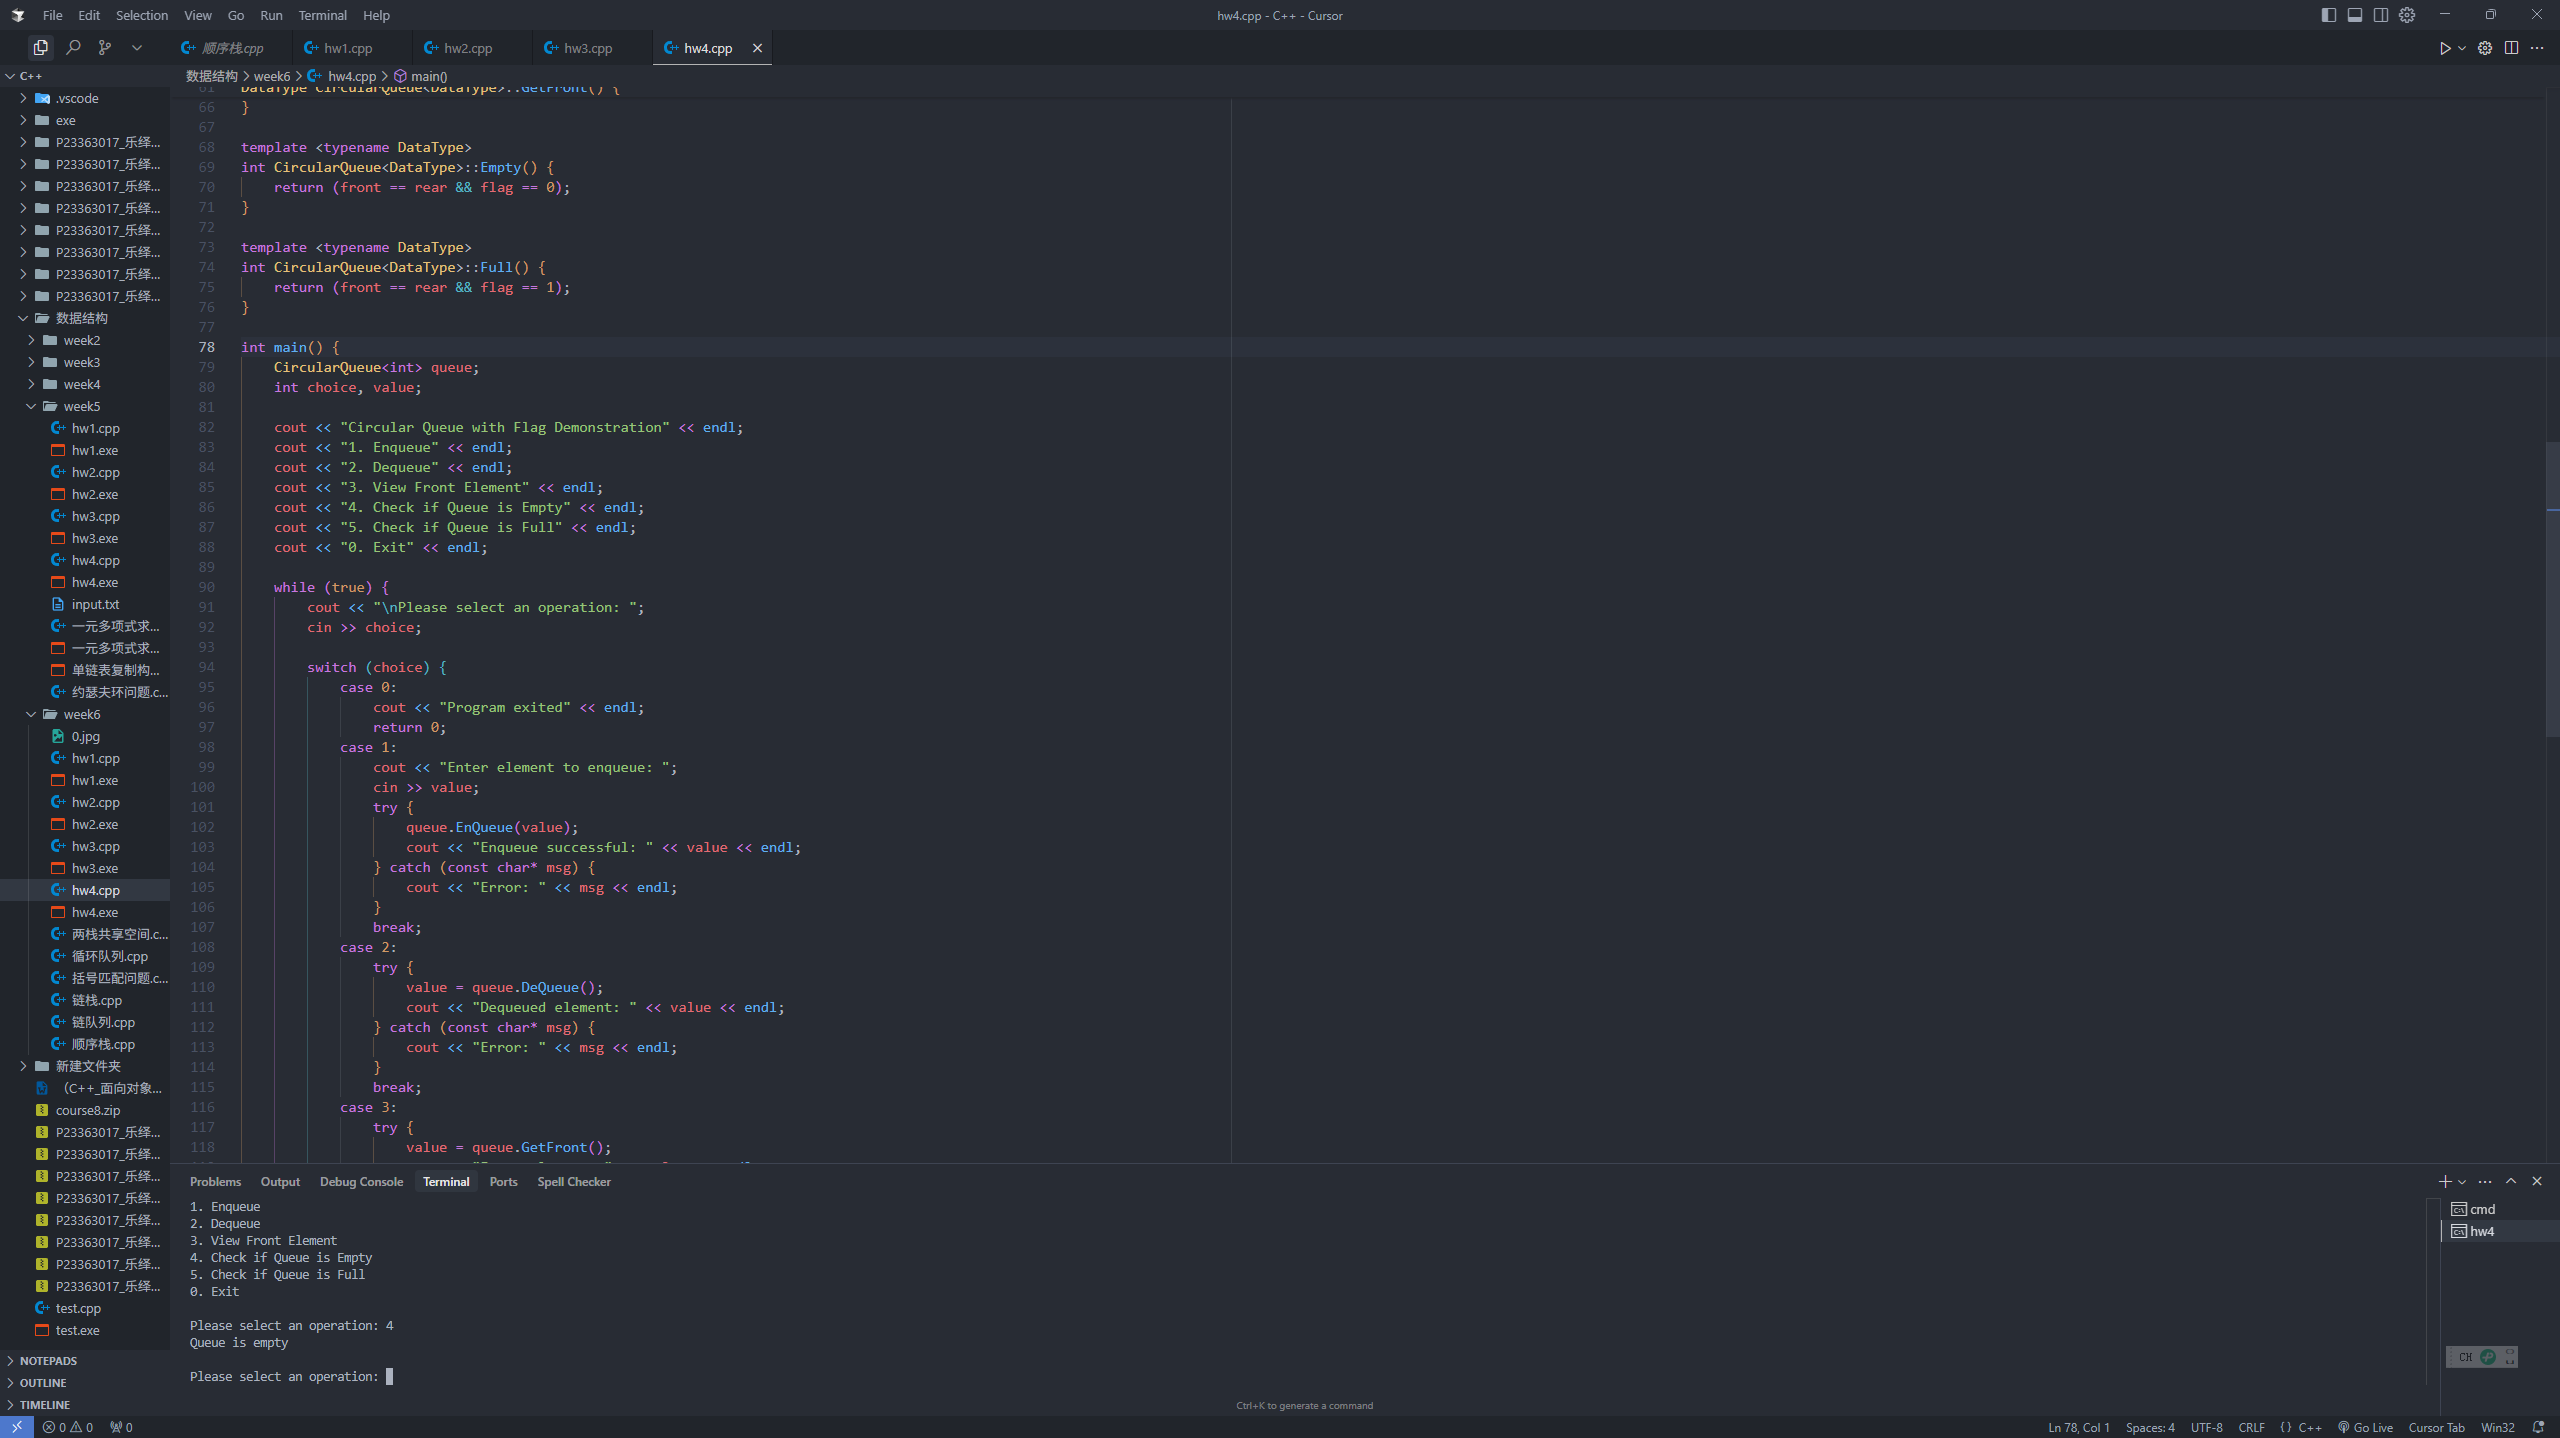
\includegraphics[width=\textwidth]{3-实验报告6-2025041423.png}
% \caption{}
\label{}
\end{figure}

\begin{lstlisting}[language=C++]
#include <iostream>

using namespace std;

  

const int QueueSize = 100;  // 队列的最大容量

  

// 带标志位的循环队列类定义

template <typename DataType>

class CircularQueue {

public:

    CircularQueue();             // 构造函数

    ~CircularQueue();            // 析构函数

    void EnQueue(DataType x);    // 入队操作

    DataType DeQueue();          // 出队操作

    DataType GetFront();         // 获取队头元素

    int Empty();                 // 判断队列是否为空

    int Full();                  // 判断队列是否已满

private:

    DataType data[QueueSize];    // 存放队列元素的数组

    int front, rear;             // 队头和队尾指针

    int flag;                    // 标志位,0表示队空,1表示队满(当front=rear时)

};

  

// 循环队列的实现

template <typename DataType>

CircularQueue<DataType>::CircularQueue() {

    front = rear = 0;

    flag = 0;  // 初始为空队列

}

  

template <typename DataType>

CircularQueue<DataType>::~CircularQueue() {

}

  

template <typename DataType>

void CircularQueue<DataType>::EnQueue(DataType x) {

    if (front == rear && flag == 1)

        throw "队列上溢";

    data[rear] = x;

    rear = (rear + 1) % QueueSize;

    if (front == rear)  // 入队后如果front=rear,说明队列已满

        flag = 1;

}

  

template <typename DataType>

DataType CircularQueue<DataType>::DeQueue() {

    if (front == rear && flag == 0)

        throw "队列下溢";

    DataType x = data[front];

    front = (front + 1) % QueueSize;

    if (front == rear)  // 出队后如果front=rear,说明队列已空

        flag = 0;

    return x;

}

  

template <typename DataType>

DataType CircularQueue<DataType>::GetFront() {

    if (front == rear && flag == 0)

        throw "队列为空";

    return data[front];

}

  

template <typename DataType>

int CircularQueue<DataType>::Empty() {

    return (front == rear && flag == 0);

}

  

template <typename DataType>

int CircularQueue<DataType>::Full() {

    return (front == rear && flag == 1);

}

  

int main() {

    CircularQueue<int> queue;

    int choice, value;

    cout << "Circular Queue with Flag Demonstration" << endl;

    cout << "1. Enqueue" << endl;

    cout << "2. Dequeue" << endl;

    cout << "3. View Front Element" << endl;

    cout << "4. Check if Queue is Empty" << endl;

    cout << "5. Check if Queue is Full" << endl;

    cout << "0. Exit" << endl;

    while (true) {

        cout << "\nPlease select an operation: ";

        cin >> choice;

        switch (choice) {

            case 0:

                cout << "Program exited" << endl;

                return 0;

            case 1:

                cout << "Enter element to enqueue: ";

                cin >> value;

                try {

                    queue.EnQueue(value);

                    cout << "Enqueue successful: " << value << endl;

                } catch (const char* msg) {

                    cout << "Error: " << msg << endl;

                }

                break;

            case 2:

                try {

                    value = queue.DeQueue();

                    cout << "Dequeued element: " << value << endl;

                } catch (const char* msg) {

                    cout << "Error: " << msg << endl;

                }

                break;

            case 3:

                try {

                    value = queue.GetFront();

                    cout << "Front element: " << value << endl;

                } catch (const char* msg) {

                    cout << "Error: " << msg << endl;

                }

                break;

            case 4:

                if (queue.Empty())

                    cout << "Queue is empty" << endl;

                else

                    cout << "Queue is not empty" << endl;

                break;

            case 5:

                if (queue.Full())

                    cout << "Queue is full" << endl;

                else

                    cout << "Queue is not full" << endl;

                break;

            default:

                cout << "Invalid choice, please try again" << endl;

        }

    }

    return 0;

}
\end{lstlisting}